% !TeX root = ../libro.tex
% !TeX encoding = utf8

\chapter{Gráficas con los tiempos de ejecución de los algoritmos}\label{ap:apendice2}

\section{BFS}

\begin{figure}[!htb]
	\centering
	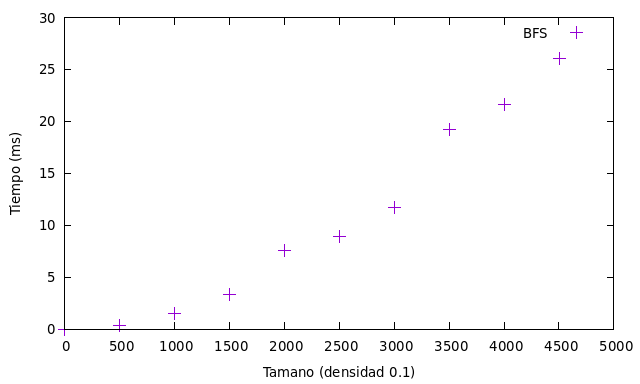
\includegraphics[width=10cm]{./Tiempos_Ejecucion/Tiempos_BFS_0.1}
	
	\caption{Tiempos de ejecución BFS.}
	\label{fig:tiempos_BFS}
\end{figure}

\section{Dijkstra}

\begin{figure}[!htb]
	\centering
	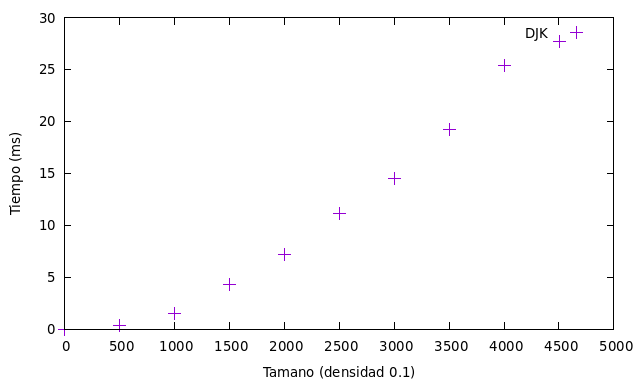
\includegraphics[width=10cm]{./Tiempos_Ejecucion/Tiempos_DJK_0.1}
	
	\caption{Tiempos de ejecución Dijkstra.}
	\label{fig:tiempos_DJK}
\end{figure}

\section{Bellman-Ford}

\begin{figure}[!htb]
	\centering
	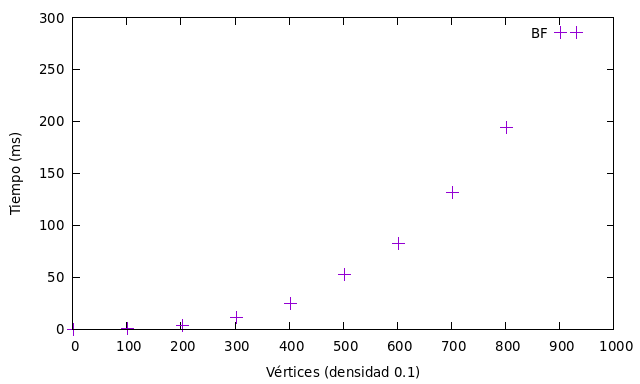
\includegraphics[width=10cm]{./Tiempos_Ejecucion/Tiempos_BF}
	
	\caption{Tiempos de ejecución Bellman-Ford.}
	\label{fig:tiempos_BF}
\end{figure}

\section{Algoritmo de matrices lento}

\begin{figure}[!htb]
	\centering
	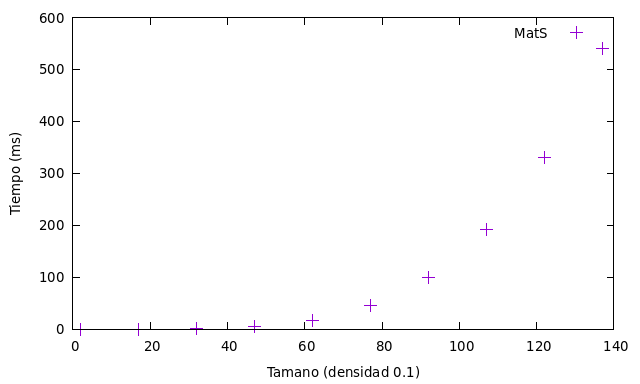
\includegraphics[width=10cm]{./Tiempos_Ejecucion/Tiempos_MatS}
	
	\caption{Tiempos de ejecución algoritmo de matrices lento.}
	\label{fig:tiempos_MatS}
\end{figure}

\newpage

\section{Algoritmo de matrices rápido}

\begin{figure}[!htb]
	\centering
	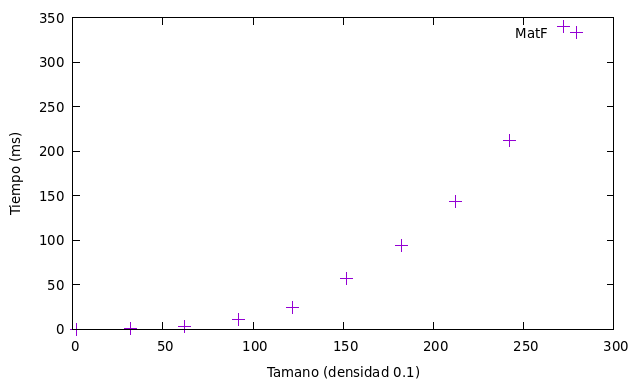
\includegraphics[width=10cm]{./Tiempos_Ejecucion/Tiempos_MatF}
	
	\caption{Tiempos de ejecución algoritmo de matrices rápido.}
	\label{fig:tiempos_MatF}
\end{figure}

\section{Floyd-Warshall}

\begin{figure}[!htb]
	\centering
	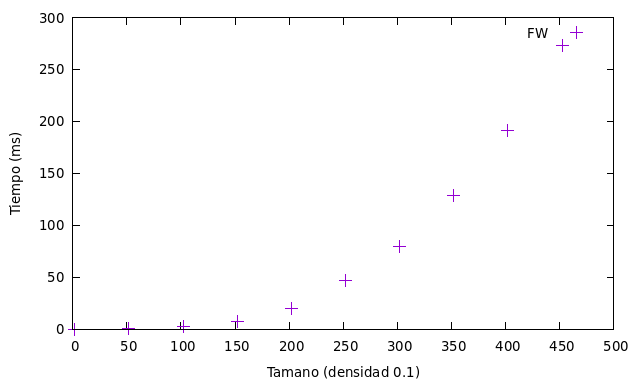
\includegraphics[width=10cm]{./Tiempos_Ejecucion/Tiempos_FW}
	
	\caption{Tiempos de ejecución Floyd-Warshall.}
	\label{fig:tiempos_FW}
\end{figure}

\newpage

\section{Todos los algoritmos}

\begin{figure}[!htb]
	\centering
	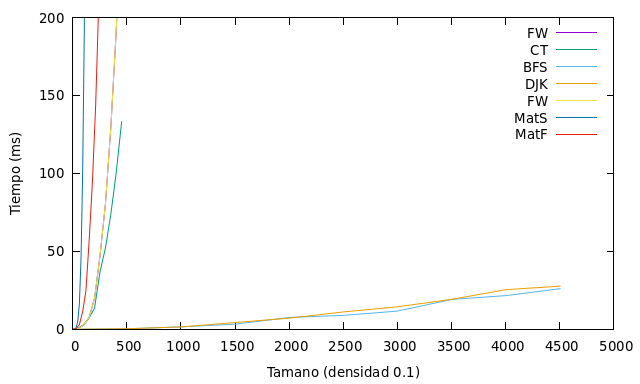
\includegraphics[width=10cm]{./Tiempos_Ejecucion/Tiempos_Todos}
	
	\caption{Tiempos de ejecución de todos los algoritmos.}
	\label{fig:tiempos_Todos}
\end{figure}


\endinput
%------------------------------------------------------------------------------------
% FIN DEL APÉNDICE. 
%------------------------------------------------------------------------------------
